\documentclass[12pt,a4paper]{article}

% ============================================
% DOCUMENT FORMAT - PROFESSOR'S TEMPLATE
% ============================================

\usepackage[a4paper,margin=1in]{geometry}
\setlength\parindent{0pt}

\usepackage{mathptmx}
\usepackage{amsmath,amssymb}
\usepackage[T1]{fontenc}
\usepackage[utf8]{inputenc}
\usepackage{textcomp}

% ============================================
% TABLES, FIGURES AND REFERENCES
% ============================================

\usepackage{graphicx}
\graphicspath{{RQ1/figures/rq1/}{RQ2/figures/rq2/}{RQ3/figures/rq3/}{RQ4/figures/rq4/}{RQ5/figures/rq5/}{output/gephi/report/}}
\usepackage{booktabs}
\usepackage{float}
\usepackage{caption}
\usepackage{hyperref}
\usepackage{url}

% Numeri di matricola: NON versionati, il repository e' pubblico.
% Stanno in matricole.tex (ignorato da git) e compaiono solo nella versione
% di consegna:
%   latexmk -pdf -jobname=RELAZIONE-consegna -usepretex='\def\consegna{}' RELAZIONE.TEX
\ifdefined\consegna
  \input{matricole.tex}
\else
  \newcommand{\matricola}[1]{}
\fi

% ============================================
% TITLE AND AUTHORS
% ============================================

\title{
Does Structure Predict?\\
A Social Network Analysis of Jury and Televote
Voting in the Eurovision Song Contest,
2016--2026
}

\author{
Luigi Botrugno, Laurea Magistrale in Informatica
(curr. C)\matricola{Botrugno}\\
Daniela Fabrizio, Laurea Magistrale in Informatica
(curr. B)\matricola{Fabrizio}\\
Sofia Musa, Laurea Magistrale in Informatica
(curr. B)\matricola{Musa}\\
Simone Samoggia, Laurea Magistrale in Informatica
(curr. C)\matricola{Samoggia}
}

\date{}

% ============================================
% DOCUMENT
% ============================================

\begin{document}

\maketitle

% ============================================
% 1. INTRODUCTION
% ============================================

\section{Introduction}
\label{introduction}


The Eurovision Song Contest (ESC) is an annual international
music competition in which participating countries award
points to songs representing other nations. Beyond its
musical dimension, the contest provides an interesting
setting for studying collective preferences and recurring
voting patterns. Previous research has identified
geographical, cultural, and political influences on voting
behaviour, suggesting that the distribution of points may
reflect more than musical preferences alone
\cite{ginsburgh2008}.

From a Social Network Analysis (SNA) perspective,
Eurovision can be represented as a directed, weighted
network in which countries are nodes and voting
relationships are edges. An edge from country $i$ to
country $j$ represents the points awarded by $i$ to $j$.
This representation makes it possible to investigate
structural properties such as reciprocity, transitivity,
community formation, centrality, and the persistence
of voting relationships over time.

Since 2016, jury and public votes have been reported
separately, providing two comparable voting networks
for each edition. This study analyses ten Grand Finals
between 2016 and 2026, excluding the cancelled 2020
edition, for a total of twenty networks. The two voting
systems operate under comparable rules but may exhibit
different structural patterns.

The aim of this project is to examine how these
patterns differ between juries and televoters, whether
they persist across editions, and to what extent
historical voting relationships and network structures
can help predict future voting behaviour. Particular
attention is given to distinguishing observed structural
patterns from effects arising from the contest's voting
constraints, using appropriate null models and
temporal evaluation.



% ============================================
% 2. PROBLEM AND MOTIVATION
% ============================================

\section{Problem and Motivation}
\label{problem-and-motivation}


Voting patterns in the Eurovision Song Contest have long
raised questions about the influence of geographical,
cultural, and historical relationships between countries.
Recurring exchanges of points are often interpreted
as evidence of regional alliances or shared preferences.
However, identifying such patterns does not necessarily
mean that they are statistically meaningful or useful
for predicting future voting behaviour.

The main challenge is to distinguish genuine network
structures from patterns that arise naturally from the
contest's voting rules. Each country distributes a fixed
set of scores among eligible finalists, while some
countries receive substantially more points than others.
Consequently, observed reciprocity, clustering, or
community structures may partly reflect popularity
and voting opportunities rather than specific
relationships between countries.

To investigate these issues, the project addresses five
research questions:

\begin{itemize}
    \item \textbf{RQ1 -- Reciprocity, transitivity,
    and persistence:}
    Do jury and televote networks differ in reciprocal
    and triadic voting patterns, and how persistent
    are these relationships across editions?

    \item \textbf{RQ2 -- Communities and homophily:}
    Do voting communities correspond to geographical
    or linguistic groups, and do juries and televoters
    exhibit different levels of within-group preference?

    \item \textbf{RQ3 -- Prestige, concentration,
    and bridging:}
    How concentrated is voting support, and to what
    extent do successful countries receive support
    from within or beyond their geographical and
    cultural groups?

    \item \textbf{RQ4 -- Similarity and temporal stability:}
    How similar are jury and televote networks within
    the same edition, and how stable are their voting
    patterns across editions?

    \item \textbf{RQ5 -- Predictive value of network
    structures:}
    Do geographical, linguistic, and community
    relationships improve the prediction of strong
    votes beyond historical popularity and
    pairwise voting history?
\end{itemize}

These questions examine voting behaviour at different
levels: local relationships and triadic structures,
community formation, the distribution of support,
temporal stability, and predictive performance.

The project contributes to the study of voting networks
by comparing two voting systems under similar rules,
evaluating structural patterns against appropriate
null models, and testing whether relationships
identified in historical networks provide useful
information for future predictions.

Ultimately, the study aims to distinguish between
network patterns that describe past voting behaviour
and those that offer additional predictive value.



% ============================================
% 3. DATASETS
% ============================================

\section{Datasets}
\label{datasets}


The dataset used in this study comes from the public
EurovisionAPI repository \cite{eurovisionapi}, which provides voting results
for the Eurovision Song Contest in a machine-readable
format. We analyse the Grand Finals from 2016 to 2026,
excluding 2020, when the contest was cancelled.
For each of the ten editions, jury and televote results
are considered separately, producing a total of
20 directed, weighted networks.

Each network is represented by an adjacency matrix
$W^{(t,l)}$, where $t$ identifies the edition and
$l \in \{\mathrm{jury}, \mathrm{public}\}$ identifies
the voting layer. An entry $W_{ij}^{(t,l)}$ corresponds
to the points awarded by country $i$ to country $j$.
Under the Eurovision voting system, each national
ballot assigns the scores $1,\ldots,8,10,12$ to
ten distinct finalists, distributing 58 points
in total.

A crucial distinction is made between eligible
and ineligible voting relationships. An eligible
dyad with weight zero indicates that a country
could have awarded points to another country
but did not. An ineligible dyad represents an
impossible vote, such as voting for oneself or
awarding points to a non-finalist. Eligibility
masks are therefore maintained separately from
the adjacency matrices and used throughout the
analyses to avoid treating impossible votes as
observed zeros.

The dataset covers 45 countries across the
considered period, although participation and
finalist status vary between editions. Countries
eliminated before the final may still cast votes,
but only finalists can receive them. The
Rest of the World vote (WLD), introduced in
2023 as an additional public ballot, is excluded
because it does not represent an individual country
and cannot be assigned geographical or linguistic
attributes.

Additional country-level attributes are used
to investigate geographical and cultural
relationships. These include UN M49 subregions,
broad language-family classifications, and
alternative cultural groupings. Multilingual
countries may belong to more than one language
family.

The original voting records are transformed into
CSV adjacency matrices, accompanied by country
attributes and eligibility information. Data
processing and analysis are performed in Python,
using libraries including NumPy, NetworkX
\cite{hagberg2008}, and Matplotlib; network
figures are drawn with Gephi. The resulting datasets, scripts,
and analytical outputs are publicly available in the
project repository \cite{projectrepo} to support reproducibility.



% ============================================
% 4. VALIDITY AND RELIABILITY
% ============================================

\section{Validity and Reliability}
\label{validity-and-reliability-not-needed-for-the-project-proposal}


\textbf{Validity.}
The network representation closely follows the
Eurovision voting system: nodes represent countries,
directed edges represent awarded points, and edge
weights correspond to the official scoring scale.
Eligibility masks distinguish possible voting
relationships from structurally impossible ones,
ensuring that network measures are computed on
the appropriate set of dyads.

However, the observed votes concern songs performed
by countries rather than countries themselves.
Factors such as song quality, musical genre,
performer popularity, running order, and diaspora
composition are not explicitly modelled.
Consequently, recurring voting relationships
cannot automatically be interpreted as political
alliances or causal effects of geographical
proximity.

Country-level attributes introduce additional
limitations. UN subregions provide a relatively
coarse geographical classification, while broad
language families cannot fully capture linguistic
and cultural relationships. Alternative cultural
groupings and language classifications are
therefore considered when assessing the robustness
of geographical and linguistic patterns.

The validity of structural comparisons also depends
on the constraints imposed by the voting system.
Each ballot distributes a fixed number of points
among eligible finalists, while recipients differ
in popularity and voting opportunities.
Appropriate null models are employed to distinguish
observed patterns from structures that may arise
mechanically under these constraints.

In particular, the analyses consider voting
opportunities, recipient popularity, and temporal
dependence when evaluating structural relationships.
The predictive analysis follows a chronological
evaluation strategy, using historical information
to predict later editions and avoiding the use
of future voting outcomes during model training.

\medskip

\textbf{Reliability.}
The analysis is implemented through reproducible
Python scripts operating on versioned input
matrices and country attributes. Randomised
procedures, including community detection and
permutation-based null models, use documented
random seeds and simulation settings.

Automated checks and repeated executions are
used to verify selected analyses and ensure
consistency between computed results and their
reported values. Nevertheless, reproducibility
does not eliminate uncertainty arising from
model assumptions or from the limited number
of observed editions.

In particular, the study includes ten contest
editions, while predictive performance is
evaluated on only four subsequent finals
(2023--2026). This limits the generalisability
of temporal and predictive findings.
Accordingly, statistical conclusions are
interpreted in relation to their specific null
models, and descriptive evidence is distinguished
from broader inferential claims.



% ============================================
% 5. MEASURES AND RESULTS
% ============================================

\section{Measures and Results}
\label{measures}

% RQ1 - Reciprocity, transitivity and persistence



\subsection{RQ1: Reciprocity, Transitivity and Persistence}
\label{sec:rq1}

The first research question investigates whether jury
and televote networks differ in their local structural
patterns and whether these relationships persist
across editions.

We analyse \textit{reciprocity}, measuring the extent
to which voting relationships are mutual, and
\textit{transitivity}, measuring the tendency of
directed two-paths to form closed triangles.
Both binary and weighted configurations are
considered, with particular attention to reciprocal
exchanges of high scores (10 and 12 points).
Temporal persistence is evaluated by examining how
frequently eligible voting relationships and
configurations recur across editions.

To distinguish structural preferences from effects
induced by recipient popularity and voting
constraints, the observed differences are compared
with appropriate null models. Multiple comparisons
are adjusted using Holm's procedure.

Table~\ref{tab:rq1_results} summarises the main
annual results.

\begin{table}[htbp]
    \centering
    \caption{Mean structural measures across editions.
    Adjusted p-values refer to the jury--televote
    comparison against the corresponding null model.}
    \label{tab:rq1_results}
    \small
    \begin{tabular}{lccc}
        \toprule
        \textbf{Measure} &
        \textbf{Jury} &
        \textbf{Public} &
        \textbf{Holm $p$} \\
        \midrule
        Binary reciprocity
            & 0.461 & 0.469 & 1.000 \\
        High-score reciprocity
            & 0.136 & 0.214 & 0.027 \\
        Directed transitivity
            & 0.532 & 0.646 & 0.720 \\
        Weighted transitivity
            & 0.292 & 0.358 & 0.045 \\
        \bottomrule
    \end{tabular}
\end{table}

Binary reciprocity is nearly identical in the two
layers, indicating no clear difference in the overall
frequency of mutual voting. However, high-score
reciprocity is substantially higher in the televote
(0.214 versus 0.136), and the difference remains
significant after controlling for popularity
(Holm $p=0.027$).

Directed transitivity is also descriptively higher
in the public network, but the null model explains
most of this difference (Holm $p=0.720$).
Weighted transitivity shows a significant deviation
from the null expectation (Holm $p=0.045$),
although the observed public advantage is smaller
than expected under that reference model.

Temporal analysis reveals stronger persistence in
the televote. Fifteen reciprocal dyads appear in
every eligible edition, compared with six in the
jury networks. Similarly, 26 public dyads reach
at least 75\% of their eligible opportunities,
compared with 15 jury dyads. Repeated exchanges
of high scores are also more frequent in the
public layer. Figure~\ref{fig:rq1_reciprocal} maps
these pairs: the persistent televote pairs form
regional chains (Nordic, Baltic, Balkan and Eastern
Mediterranean), while 10 of the 15 jury pairs
cross subregions.

\begin{figure}[htbp]
    \centering
    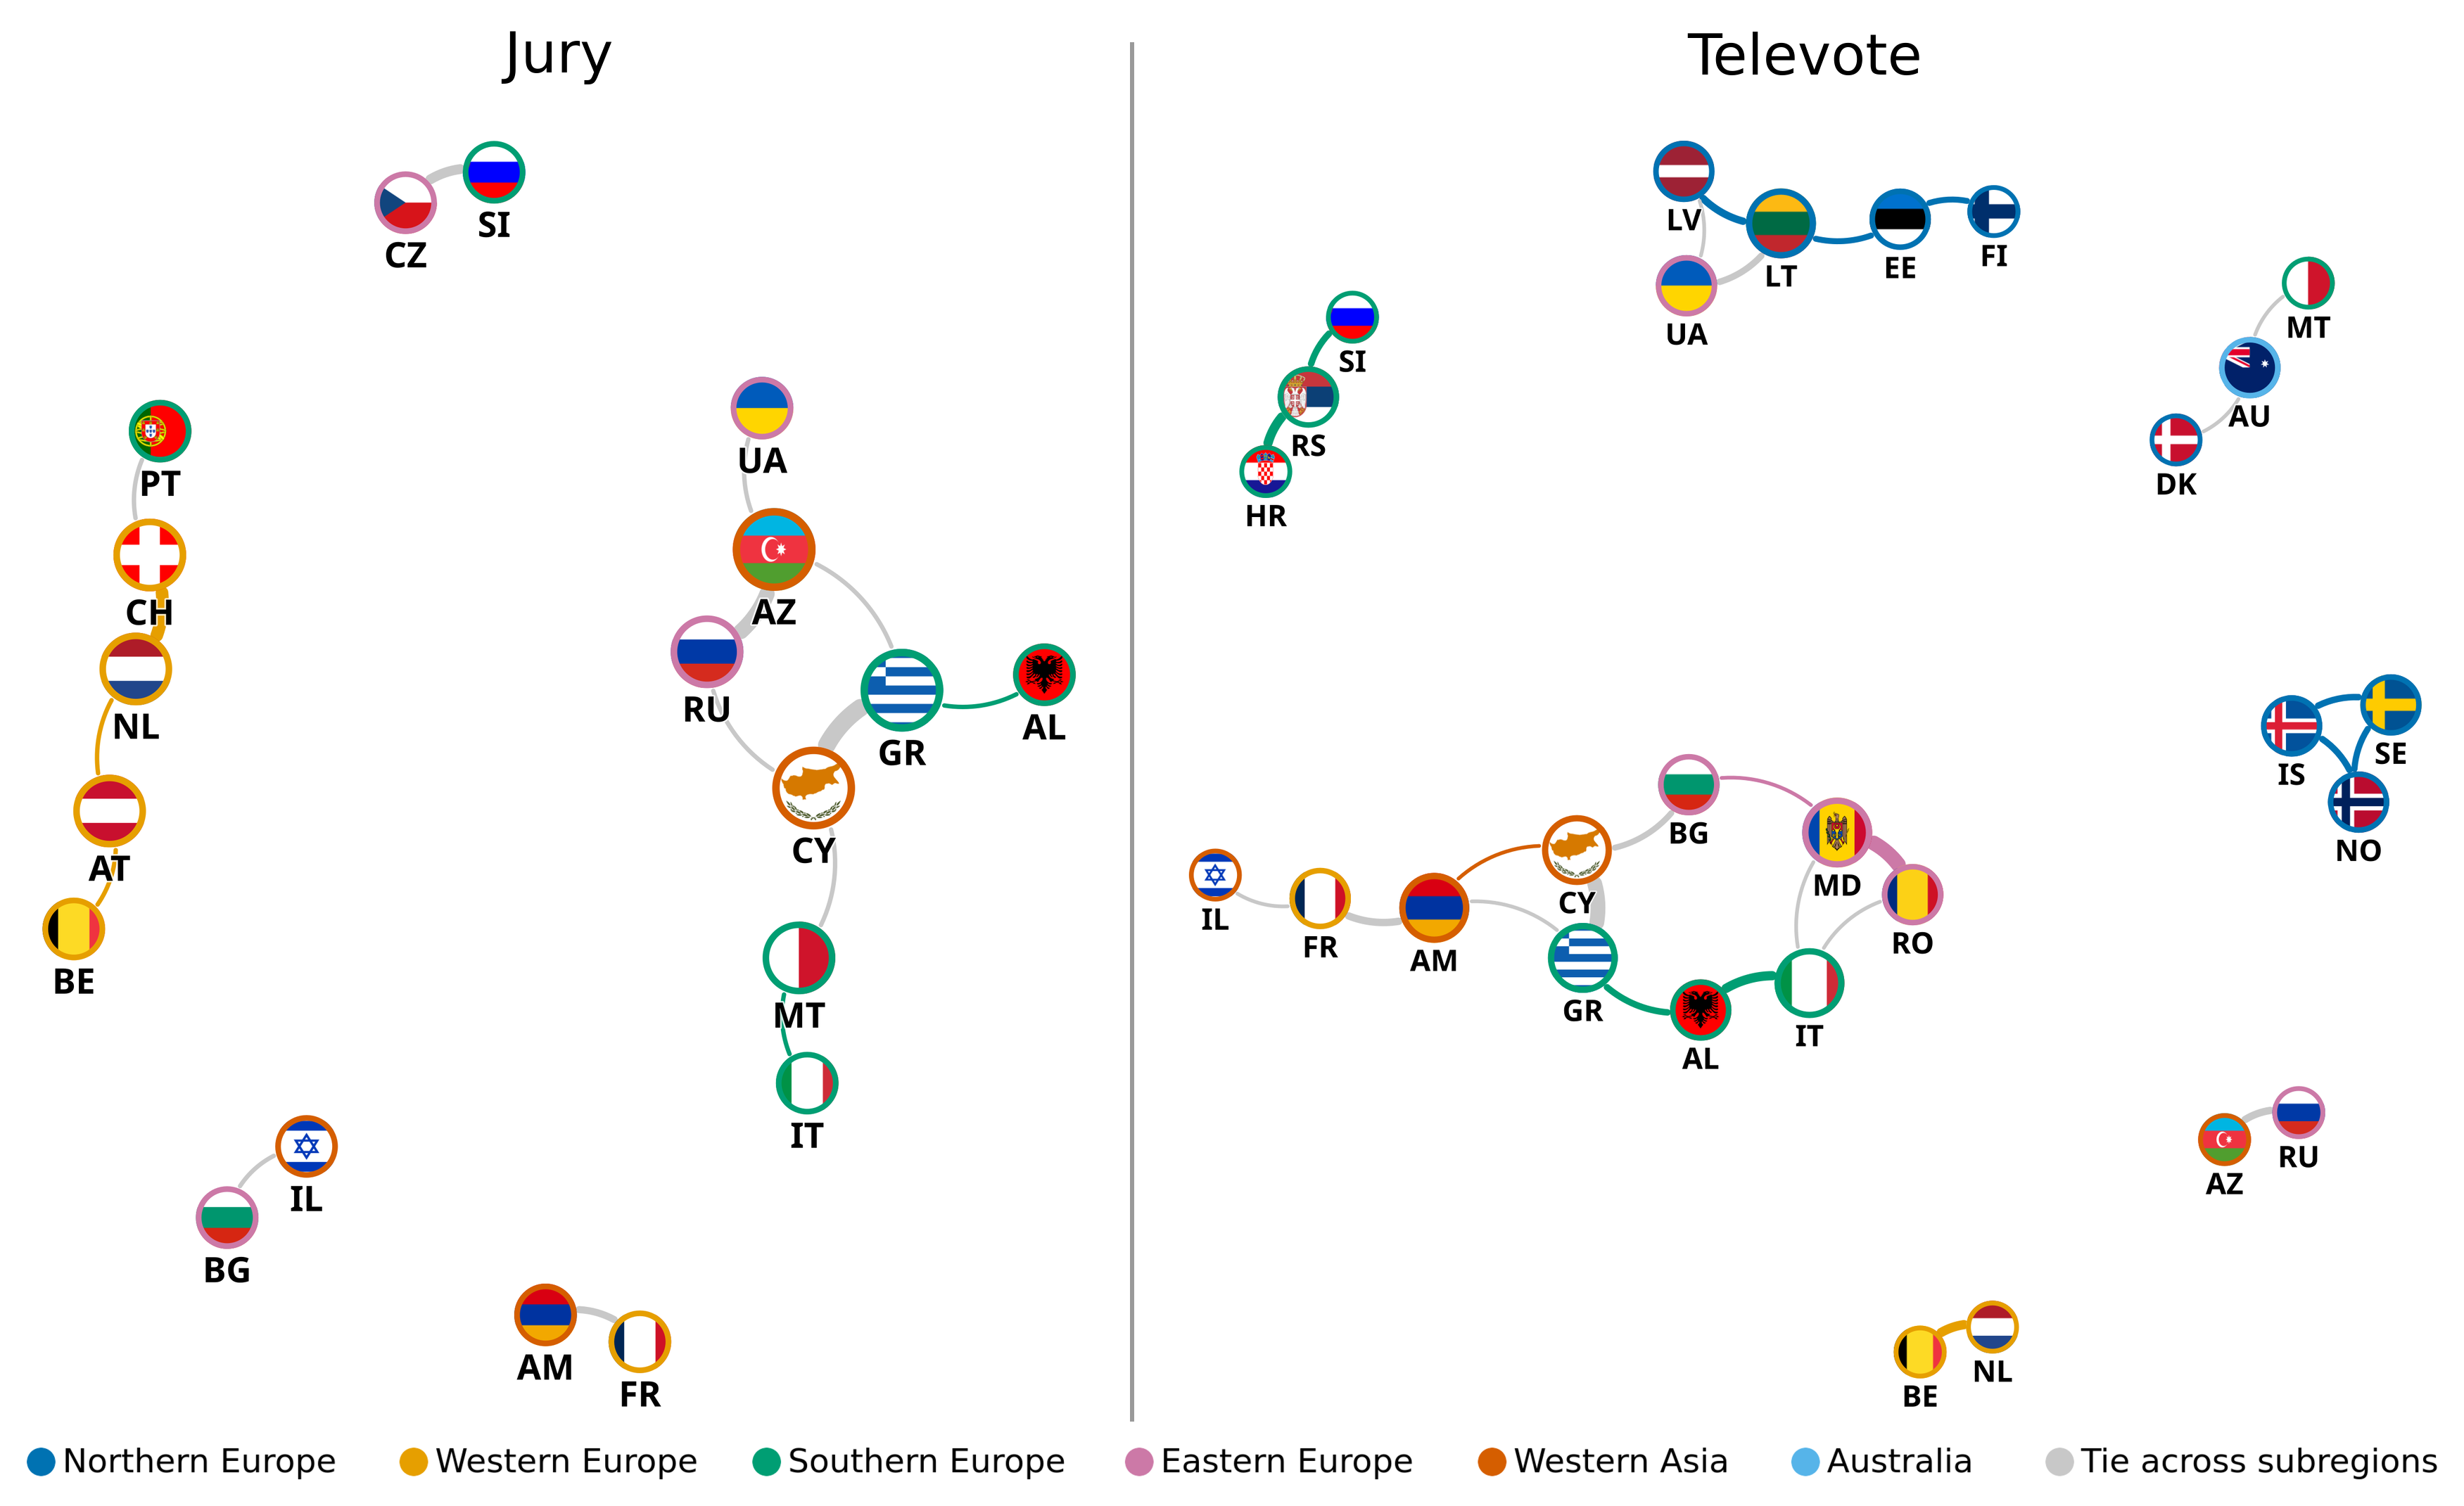
\includegraphics[width=\textwidth]
    {fig_reciprocal_ties.png}
    \caption{Pairs reciprocal in at least 75\% of
    the finals in which both were eligible (Gephi,
    ForceAtlas2). Ring colour: UN subregion; edge
    width: share of mutual 10/12-point exchanges.}
    \label{fig:rq1_reciprocal}
\end{figure}

Figure~\ref{fig:rq1_temporal} compares the observed
public--jury differences in temporal persistence
with the distributions generated under the
corresponding null model. In all three cases,
the observed differences exceed the null
expectations, indicating that the greater
persistence of reciprocal relationships in
the televote is not readily explained by
the constraints represented in that model.


\begin{figure}[htbp]
    \centering
    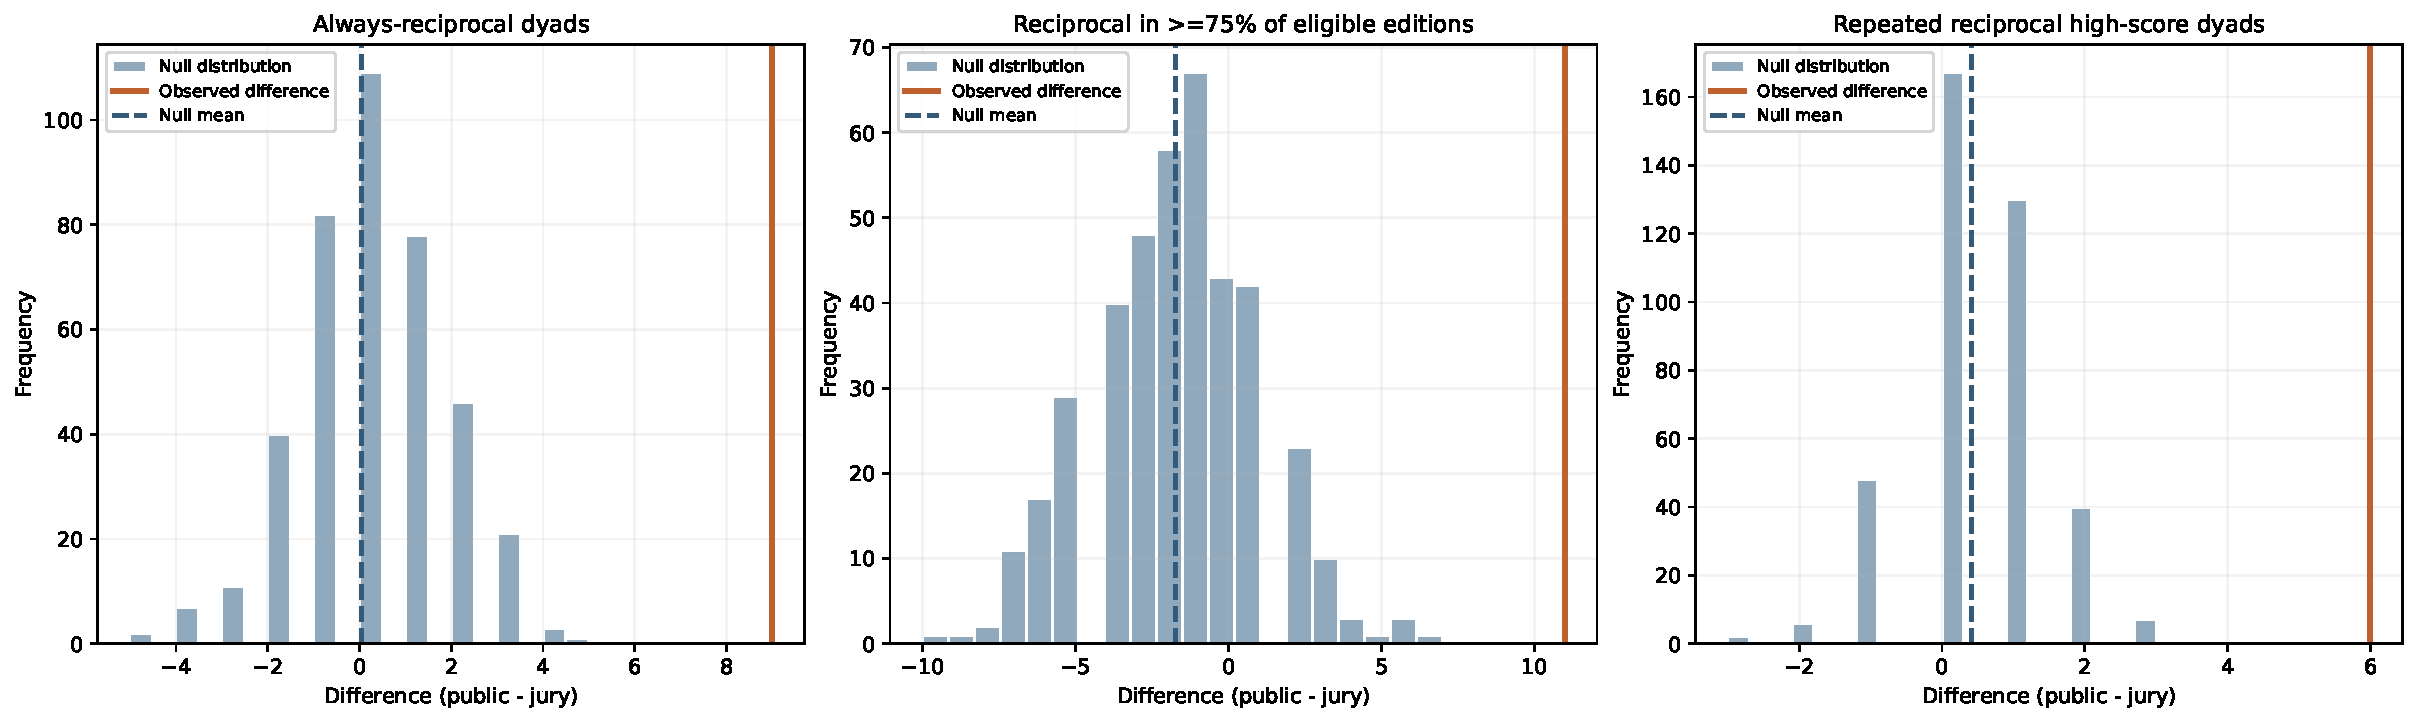
\includegraphics[width=\textwidth]
    {rq1_temporal_null_comparison.pdf}
    \caption{Temporal persistence of reciprocal voting
    relationships. Histograms show the null-model
    distributions of public--jury differences.
    Solid vertical lines indicate observed differences,
    while dashed lines indicate null-model means.
    The panels represent always-reciprocal dyads,
    dyads reciprocal in at least 75\% of eligible
    editions, and repeated reciprocal high-score
    exchanges, respectively.}
    \label{fig:rq1_temporal}
\end{figure}


Overall, jury and televote networks exhibit
similar levels of binary reciprocity, but
the public layer shows stronger high-score
reciprocity and more persistent reciprocal
relationships. Conversely, differences in
triadic closure are largely explained by
recipient popularity. These findings highlight
the importance of evaluating observed
network structures against null models
that preserve relevant voting constraints.


% RQ2 - Communities and homophily


\subsection{RQ2: Communities and Homophily}

The second research question examines whether voting
networks exhibit communities corresponding to
geographical or linguistic groups, and whether
within-group preferences differ between juries
and televoters.

Communities are identified using the Louvain
algorithm \cite{blondel2008} on an undirected, weighted projection
of each voting network. To account for stochastic
variability, multiple runs are performed and
consensus partitions are constructed. Their
agreement with geographical subregions and
language-family classifications is evaluated
using the Adjusted Rand Index (ARI) and
Normalized Mutual Information (NMI) \cite{danon2005}.

We also measure geographical and linguistic
homophily directly through voting relationships.
For each voter, the observed proportion of
within-group choices is compared with the
proportion expected among eligible recipients.
This opportunity-adjusted comparison prevents
the composition of the finalist pool from being
mistaken for a voting preference.

\begin{table}[htbp]
\centering
\caption{Mean geographical homophily measures
across the ten editions.}
\label{tab:rq2_homophily}
\small
\begin{tabular}{lcc}
\toprule
\textbf{Measure} & \textbf{Jury} & \textbf{Public} \\
\midrule
Same-subregion choices & 21.9\% & 25.1\% \\
Same-subregion points & 23.3\% & 29.5\% \\
Points per same-region choice & 6.16 & 6.86 \\
Points per other-region choice & 5.70 & 5.46 \\
\bottomrule
\end{tabular}
\end{table}

The televote exhibits stronger geographical homophily
than the jury. On average, 25.1\% of public choices
remain within the voter's subregion, compared with
21.9\% for juries and an opportunity-based expectation
of approximately 18.7\%. The difference also
appears in the distribution of points: 29.5\%
of public points go to the same subregion,
compared with 23.3\% for juries.


Figure~\ref{fig:rq2_opportunity} illustrates
the geographical differences in both recipient
selection and the intensity of awarded points
across the ten editions.


These differences concern both the selection of
recipients and the scores awarded once selected.
The public--jury difference reaches approximately
3.2 percentage points for within-subregion
choices and 6.2 percentage points for the share
of points. Both remain significant after
Holm correction ($p=0.012$).

Community detection provides complementary
evidence. The correspondence between Louvain
communities and geographical subregions is
stronger for the televote (ARI $=0.280$)
than for juries (ARI $=0.091$).
Public communities are also more reproducible
across different Louvain initialisations.

Figure~\ref{fig:rq2_strong} shows the same
pattern on the aggregate 2016--2026 networks,
dichotomised to keep only strong ties: an edge
$i \to j$ is kept when $i$ gave $j$ at least
6 points per eligible final (zeros included,
at least three finals). The televote retains
130 ties, 48\% within a subregion, and forms
visible regional clusters; the jury retains
74 ties, only 35\% within a subregion.

\begin{figure}[htbp]
    \centering
    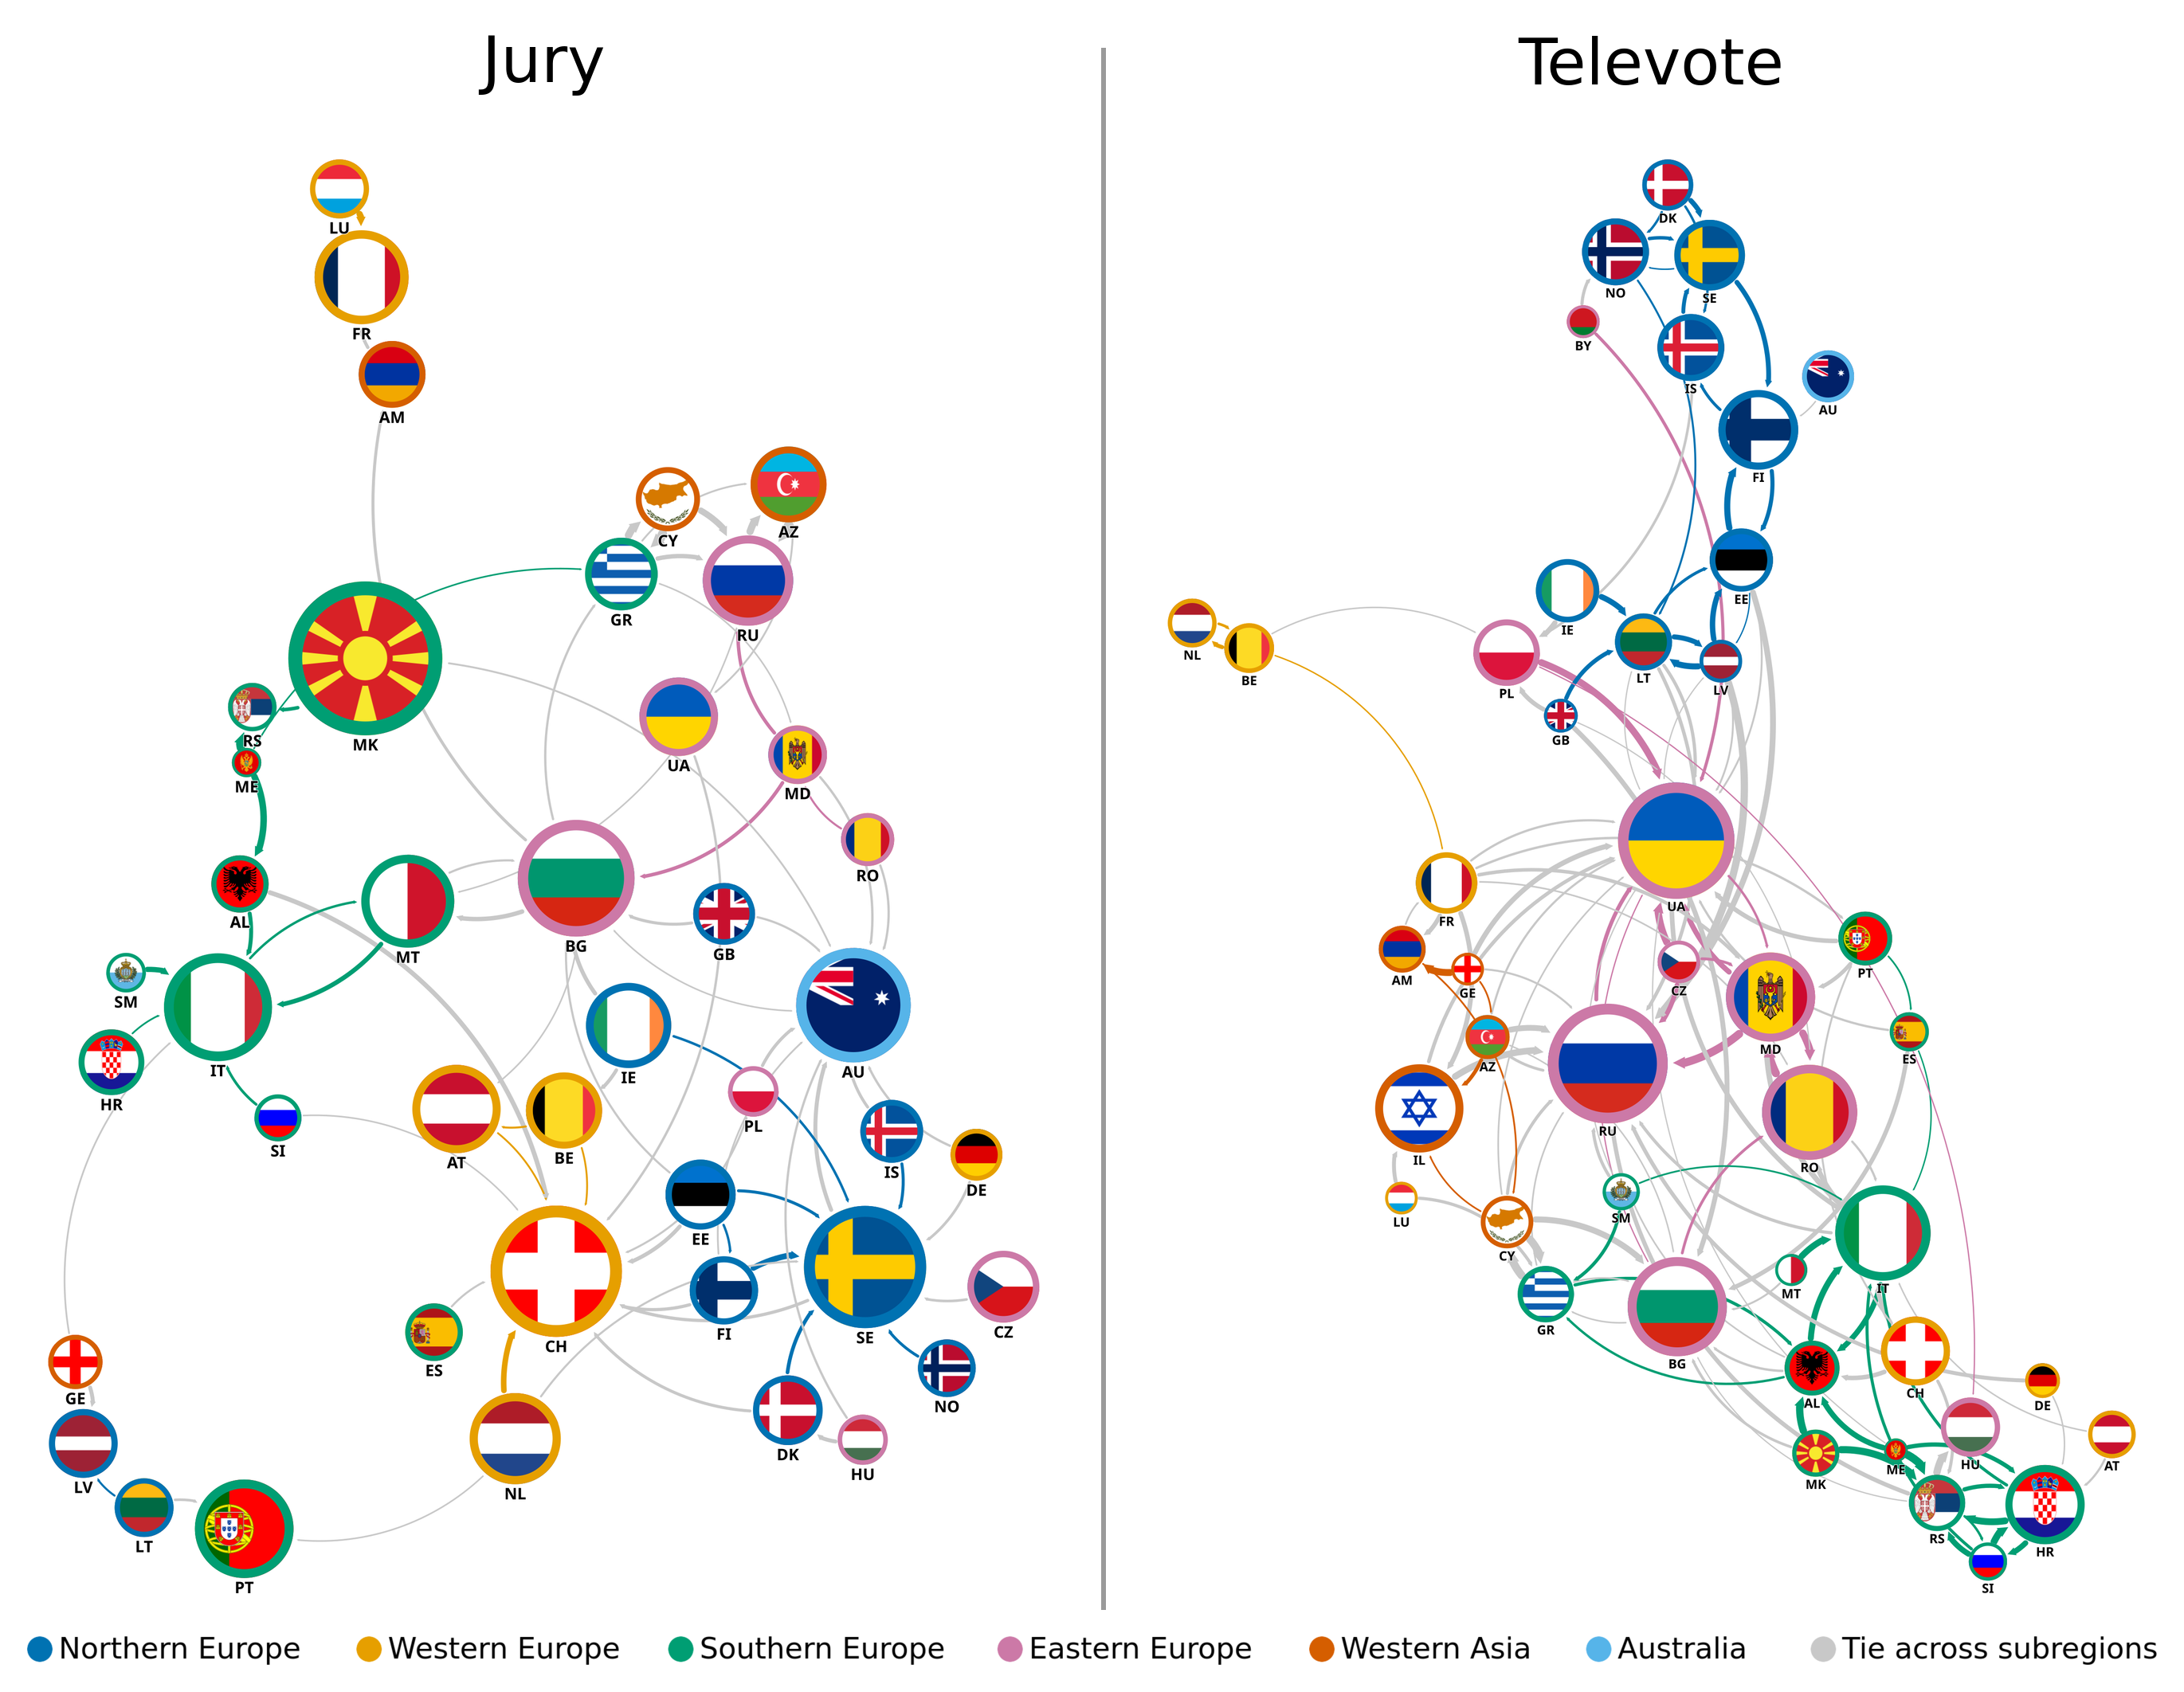
\includegraphics[width=0.75\textwidth]
    {fig_strong_ties.png}
    \caption{Strong voting ties 2016--2026
    ($\geq$6 points per eligible final; Gephi,
    ForceAtlas2). Node size: points received per
    opportunity; coloured edges stay within a
    UN subregion, grey edges cross subregions.}
    \label{fig:rq2_strong}
\end{figure}

However, modularity \cite{newman2004} alone does not establish
the presence of exceptional community structure.
Under null models that preserve relevant
network constraints, much of the observed
modularity can arise without additional
group-specific preferences.

Linguistic homophily is present but weaker,
and the evidence does not establish a clear
difference between voting layers. Overall,
the results indicate that geographical
relationships explain a larger part of
the distinction between jury and televote
networks than broad linguistic classifications.



\begin{figure}[htbp]
    \centering
    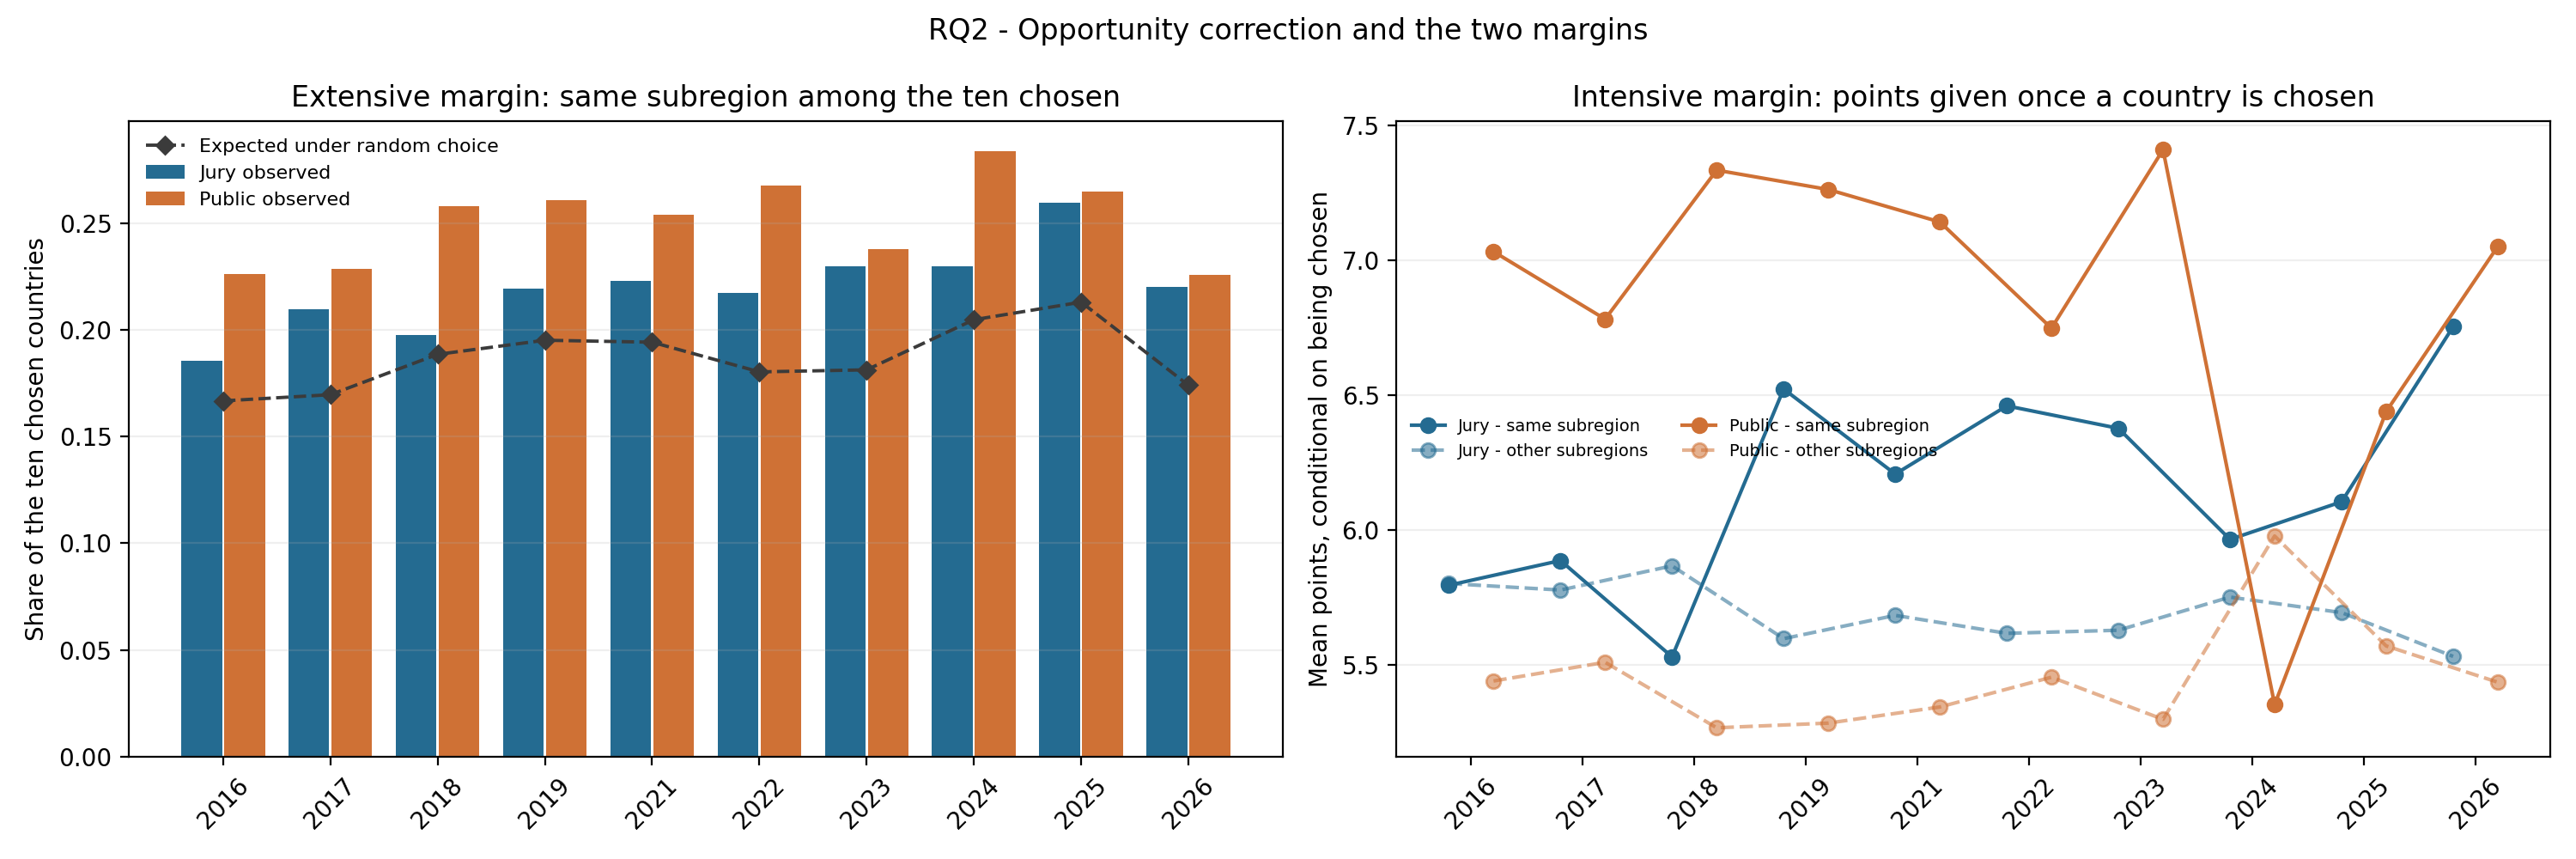
\includegraphics[width=\textwidth]
    {rq2_opportunity.png}
    \caption{Geographical homophily in jury and
    televote networks. The left panel compares
    the observed share of within-subregion
    voting choices with the expectation under
    random selection among eligible finalists.
    The right panel compares the mean points
    awarded to recipients inside and outside
    the voter's subregion, conditional on
    receiving points.}
    \label{fig:rq2_opportunity}
\end{figure}


% RQ3 - Prestige, concentration and bridging


\subsection{RQ3: Prestige, Concentration and Bridging}
\label{sec:rq3}

The third research question investigates how voting
support is distributed among finalists and whether
successful countries attract votes primarily from
their own geographical groups or from a broader
set of countries.

We measure concentration using the Gini coefficient
of received points and the share of points awarded
to the three most supported finalists. To assess
the geographical origin of support, we calculate
\textit{home excess}: the difference between the
observed share of points received from a finalist's
own subregion and the share expected from eligible
voters. We also examine the participation ratio,
which measures the diversity of geographical groups
contributing to a finalist's support.

These measures are compared with random-ballot
and popularity-preserving null models. The latter
controls for the number of voters supporting each
finalist and the total points received, helping
distinguish geographical preferences from effects
of overall popularity.

\begin{table}[htbp]
\centering
\caption{Mean concentration and geographical
support measures across editions.}
\label{tab:rq3_results}
\small
\begin{tabular}{lccc}
\toprule
\textbf{Measure} &
\textbf{Jury} &
\textbf{Public} &
\textbf{Random ballots} \\
\midrule
Gini coefficient & 0.447 & 0.538 & 0.137 \\
Top-three point share & 0.315 & 0.372 & 0.166 \\
Home excess & 0.083 & 0.193 & 0.000 \\
Participation ratio & 0.835 & 0.727 & 0.934 \\
\bottomrule
\end{tabular}
\end{table}

Voting support is considerably more concentrated
than under random allocation. The mean Gini
coefficient is 0.447 for juries and 0.538 for
the televote, indicating that public points
are distributed less evenly among finalists.
Similarly, the three most supported finalists
receive 37.2\% of public points, compared with
31.5\% of jury points.

The two layers also reward different countries:
within the same final, the Spearman correlation
between jury and public in-strength averages only
0.40 (minimum 0.21). Ukraine, Romania, Russia and
Moldova are much stronger with the televote, Malta,
Australia, Switzerland and Sweden with juries
(Figure~\ref{fig:rq3_prestige}).

\begin{figure}[htbp]
    \centering
    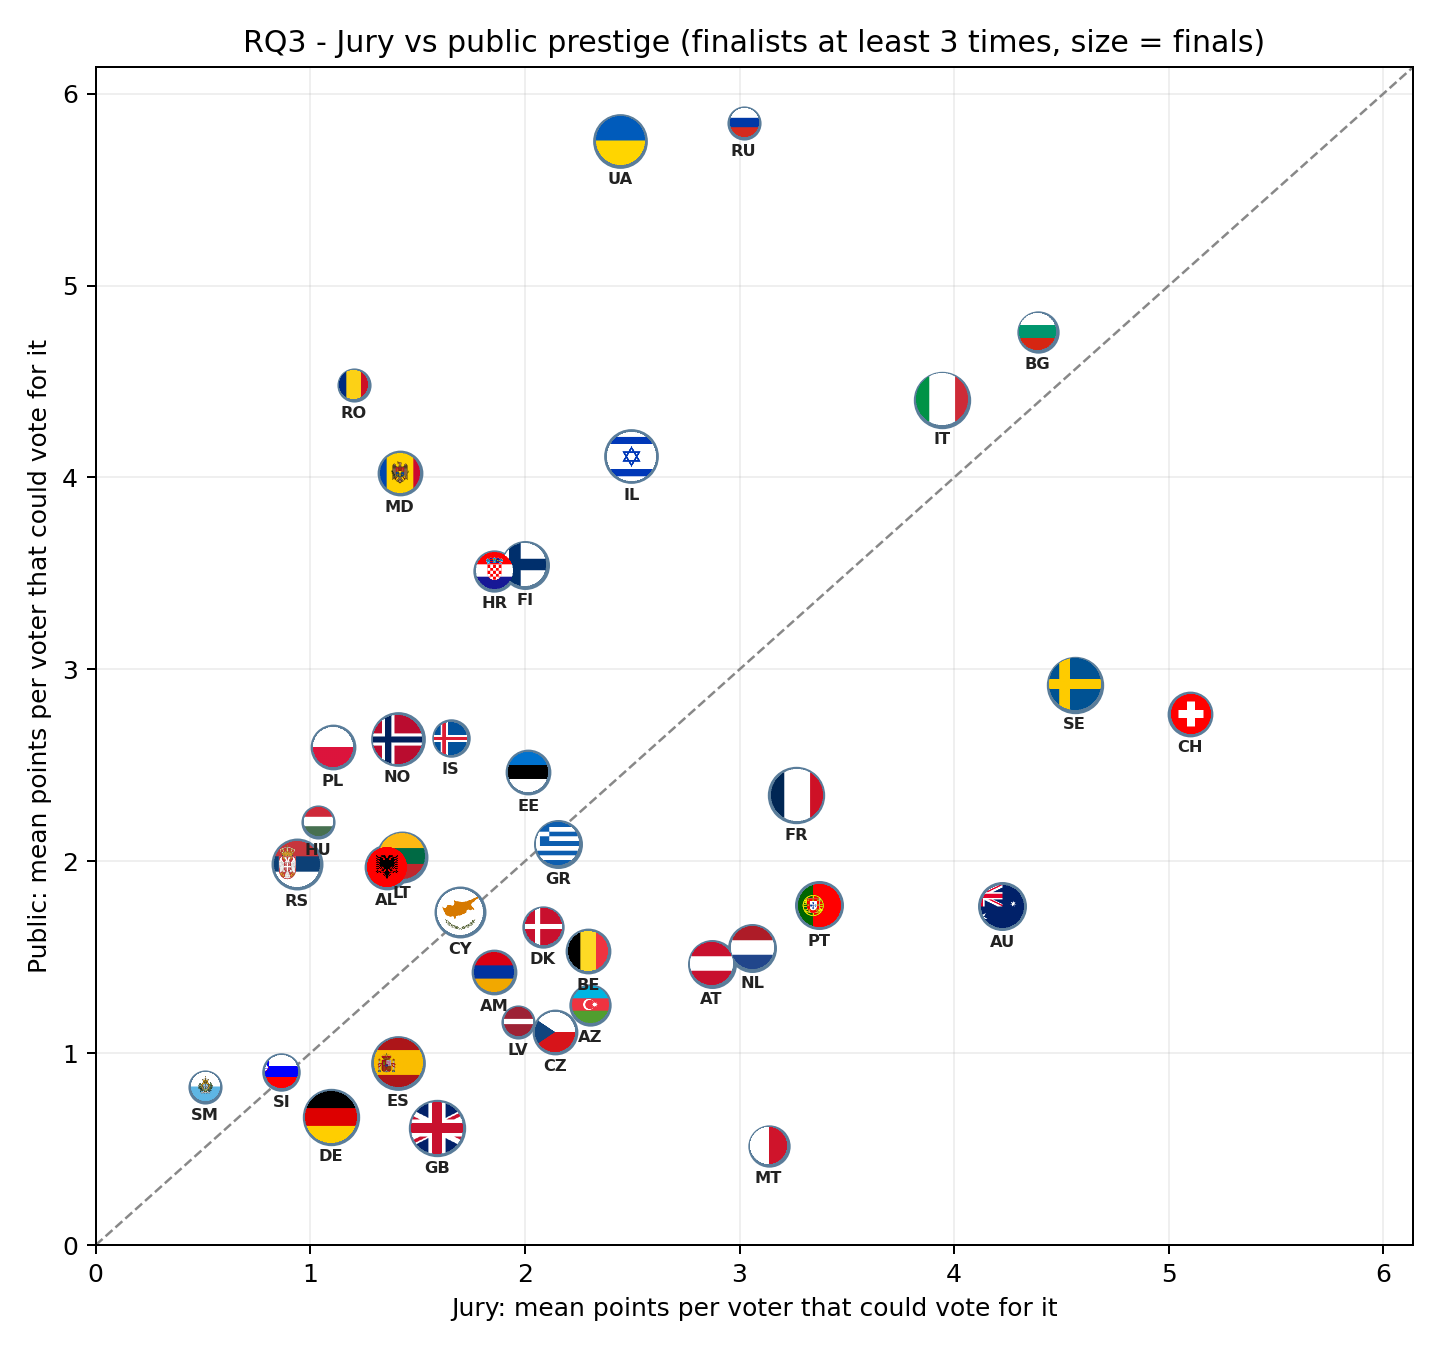
\includegraphics[width=0.75\textwidth]
    {rq3_jury_vs_public_prestige.png}
    \caption{Mean points per eligible voter received
    from juries and televoters (finalists at least
    three times; flag size: number of finals).
    Countries above the diagonal do better with
    the televote.}
    \label{fig:rq3_prestige}
\end{figure}

The televote also exhibits stronger geographical
home bias. Its mean home excess is 0.193,
compared with 0.083 for juries. This difference
remains supported by the popularity-preserving
analysis, indicating that the concentration of
support within geographical groups cannot be
explained solely by recipient popularity.


Figure~\ref{fig:rq3_popularity} compares
the observed geographical home excess
with a popularity-preserving null model.
The public layer shows a consistently
larger deviation from the null expectation,
supporting the interpretation of stronger
within-region voting preferences.


An important methodological result concerns
the relationship between prestige and the
geographical diversity of support. The observed
Spearman correlation between prestige and
participation ratio is positive in both layers
(0.717 for juries and 0.815 for the public).
However, under a null model preserving recipient
popularity, the expected correlations are
0.753 and 0.836, respectively.

Therefore, the positive correlations do not
provide independent evidence that prestigious
countries attract more geographically diverse
support. Much of the apparent relationship
arises mechanically because finalists receiving
votes from more countries also tend to receive
support from more geographical groups.

Overall, the televote concentrates support
on fewer finalists and exhibits stronger
within-region preferences. At the same time,
the analysis demonstrates that apparent
relationships between network measures must
be interpreted against null models that
preserve relevant structural constraints.



\begin{figure}[htbp]
    \centering
    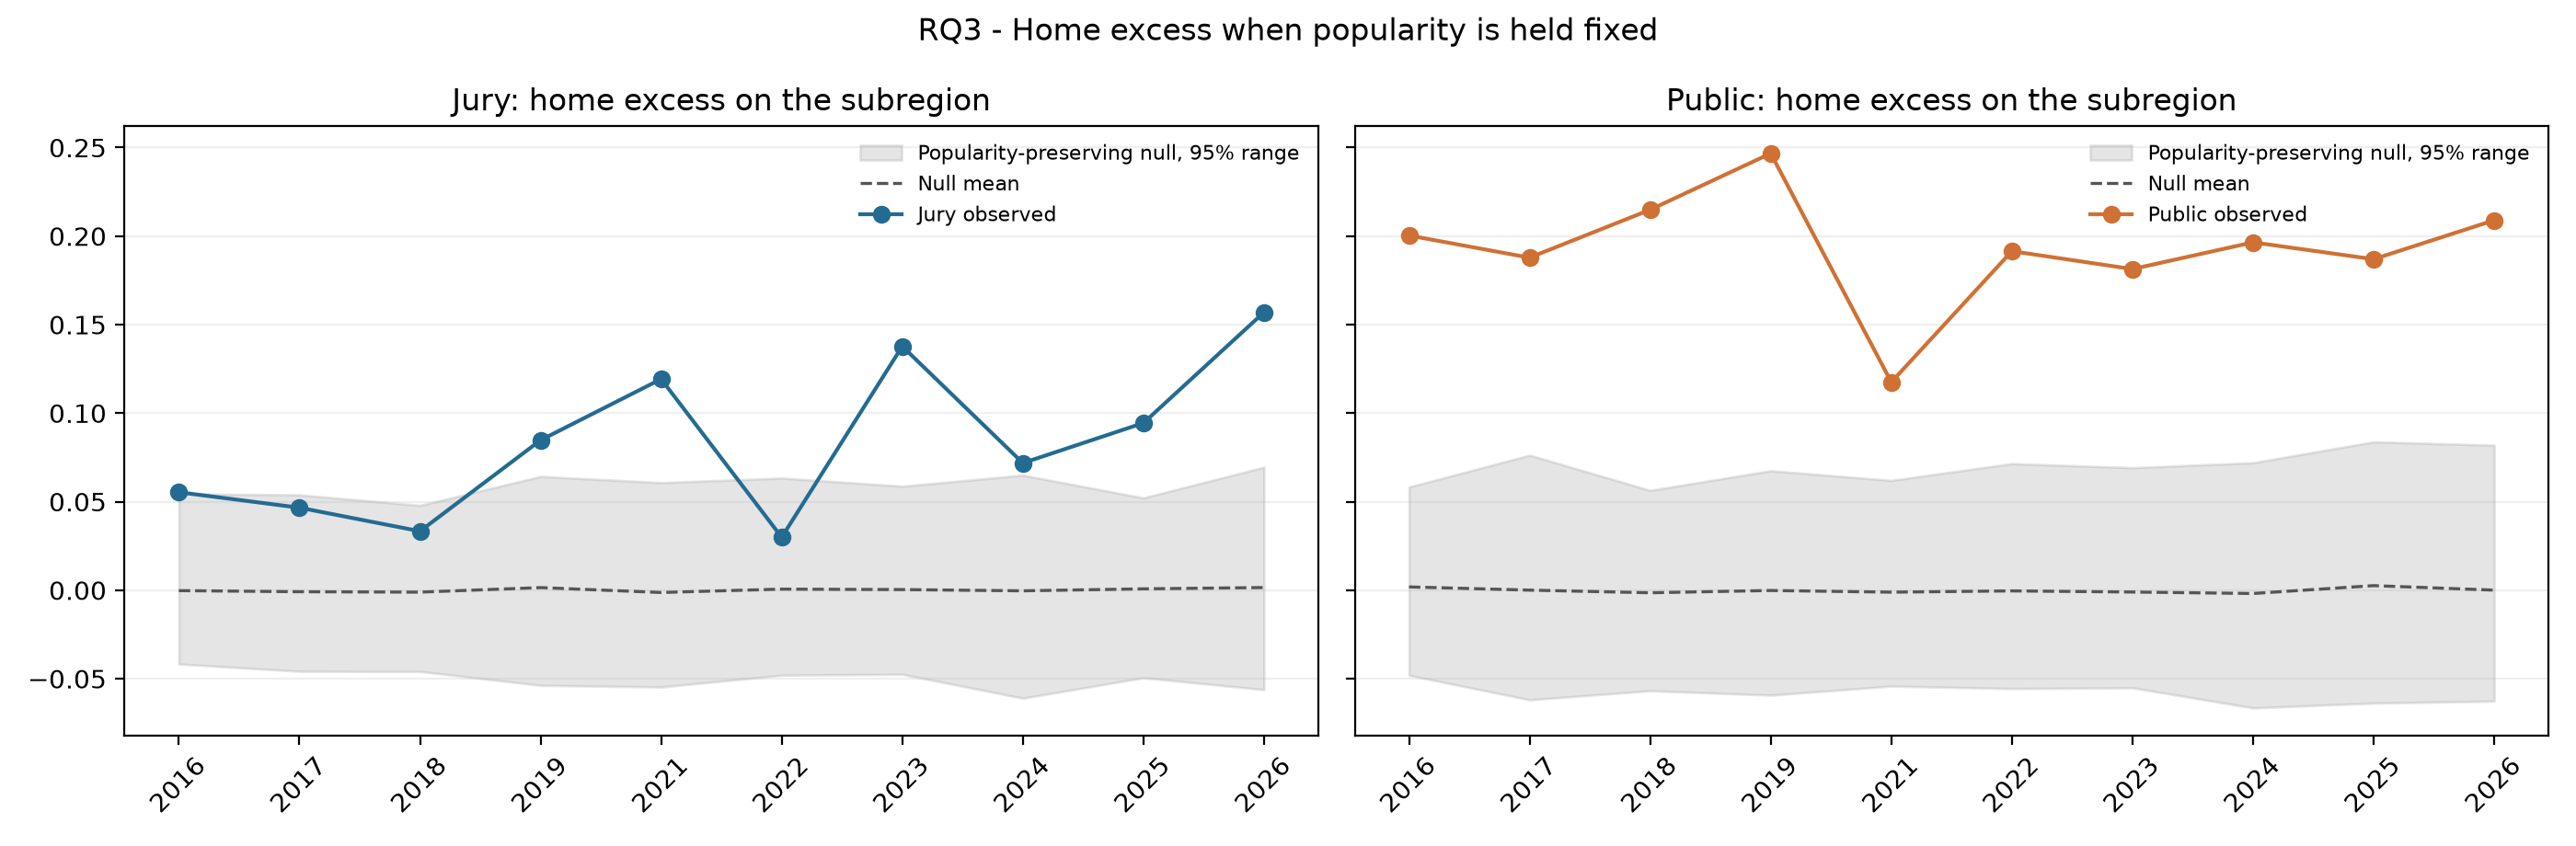
\includegraphics[width=\textwidth]
    {rq3_popularity_null.png}
    \caption{Geographical home excess under a
    popularity-preserving null model.
    Solid lines show observed home excess for
    juries and televoters across editions.
    Dashed lines indicate the mean null
    expectation, while shaded regions
    represent the central 95\% of simulated
    values. The public layer exhibits
    consistently stronger within-subregion
    support than expected under this reference.}
    \label{fig:rq3_popularity}
\end{figure}

% RQ4 - Similarity and temporal stability


\subsection{RQ4: Similarity and Temporal Stability}
\label{sec:rq4}

The fourth research question examines the agreement
between jury and televote networks within each
edition and the persistence of voting relationships
across editions.

Within-edition similarity is measured using
Spearman and Pearson correlations on eligible
dyads, together with the Jaccard index on positive
voting relationships. To distinguish dyadic
agreement from general voting tendencies, we
also calculate the Pearson correlation between
residuals obtained from an additive model with
voter and recipient fixed effects, estimated on
the common eligible dyads.

Temporal stability is evaluated by comparing
networks from different editions using the
intersection of their eligibility masks.
Particular attention is given to consecutive
editions (lag 1), with longer lags examined
descriptively.

\begin{table}[htbp]
\centering
\caption{Mean similarity between consecutive
editions (lag 1).}
\label{tab:rq4_stability}
\small
\begin{tabular}{lccc}
\toprule
\textbf{Measure} &
\textbf{Jury} &
\textbf{Public} &
\textbf{Difference} \\
\midrule
Spearman & 0.099 & 0.263 & +0.165 \\
Residual Pearson & 0.118 & 0.472 & +0.354 \\
Jaccard & 0.292 & 0.359 & +0.067 \\
\bottomrule
\end{tabular}
\end{table}

Within the same edition, jury and televote
networks exhibit moderate positive agreement:
mean Spearman correlation is 0.311, while
the Pearson correlation between fixed-effect
residuals is approximately 0.241.
The latter exceeds its permutation-based
reference in all ten editions
(Holm-adjusted $p=0.0020$).

Across consecutive editions, the televote
is substantially more stable than the jury.
The mean residual Pearson correlation is
0.472 for the public and 0.118 for juries,
a difference of approximately 0.354.
The public layer shows higher residual
correlation in all nine consecutive-edition
comparisons.


Figure~\ref{fig:rq4_temporal} illustrates
the greater temporal similarity of public
voting networks across the observed editions.
Longer-lag comparisons remain descriptive,
particularly because fewer edition pairs
are available at larger lags.


To assess temporal structure, a joint
QAP-style permutation null model
\cite{krackhardt1988} independently
reassigns country identities within their
eligible roles for each edition. The same
annual permutation is shared by jury and
televote and reused across all comparisons
involving that edition, preserving the
dependence induced by shared years.

Under this reference, the observed stability
of both layers and the public--jury difference
are unusually high (Holm-adjusted
$p=0.0006$ for each primary temporal test).

The difference remains positive when
restricting comparisons to the 130 dyads
eligible in every edition (+0.346)
and when excluding one edition at a time
(range: +0.318 to +0.374).

These findings indicate stronger persistence
of televote relationships in the observed
networks. However, the temporal permutation
test evaluates deviations from a null model
without persistent country identities;
it does not directly test equality between
two potentially persistent voting processes.


\begin{figure}[htbp]
    \centering
    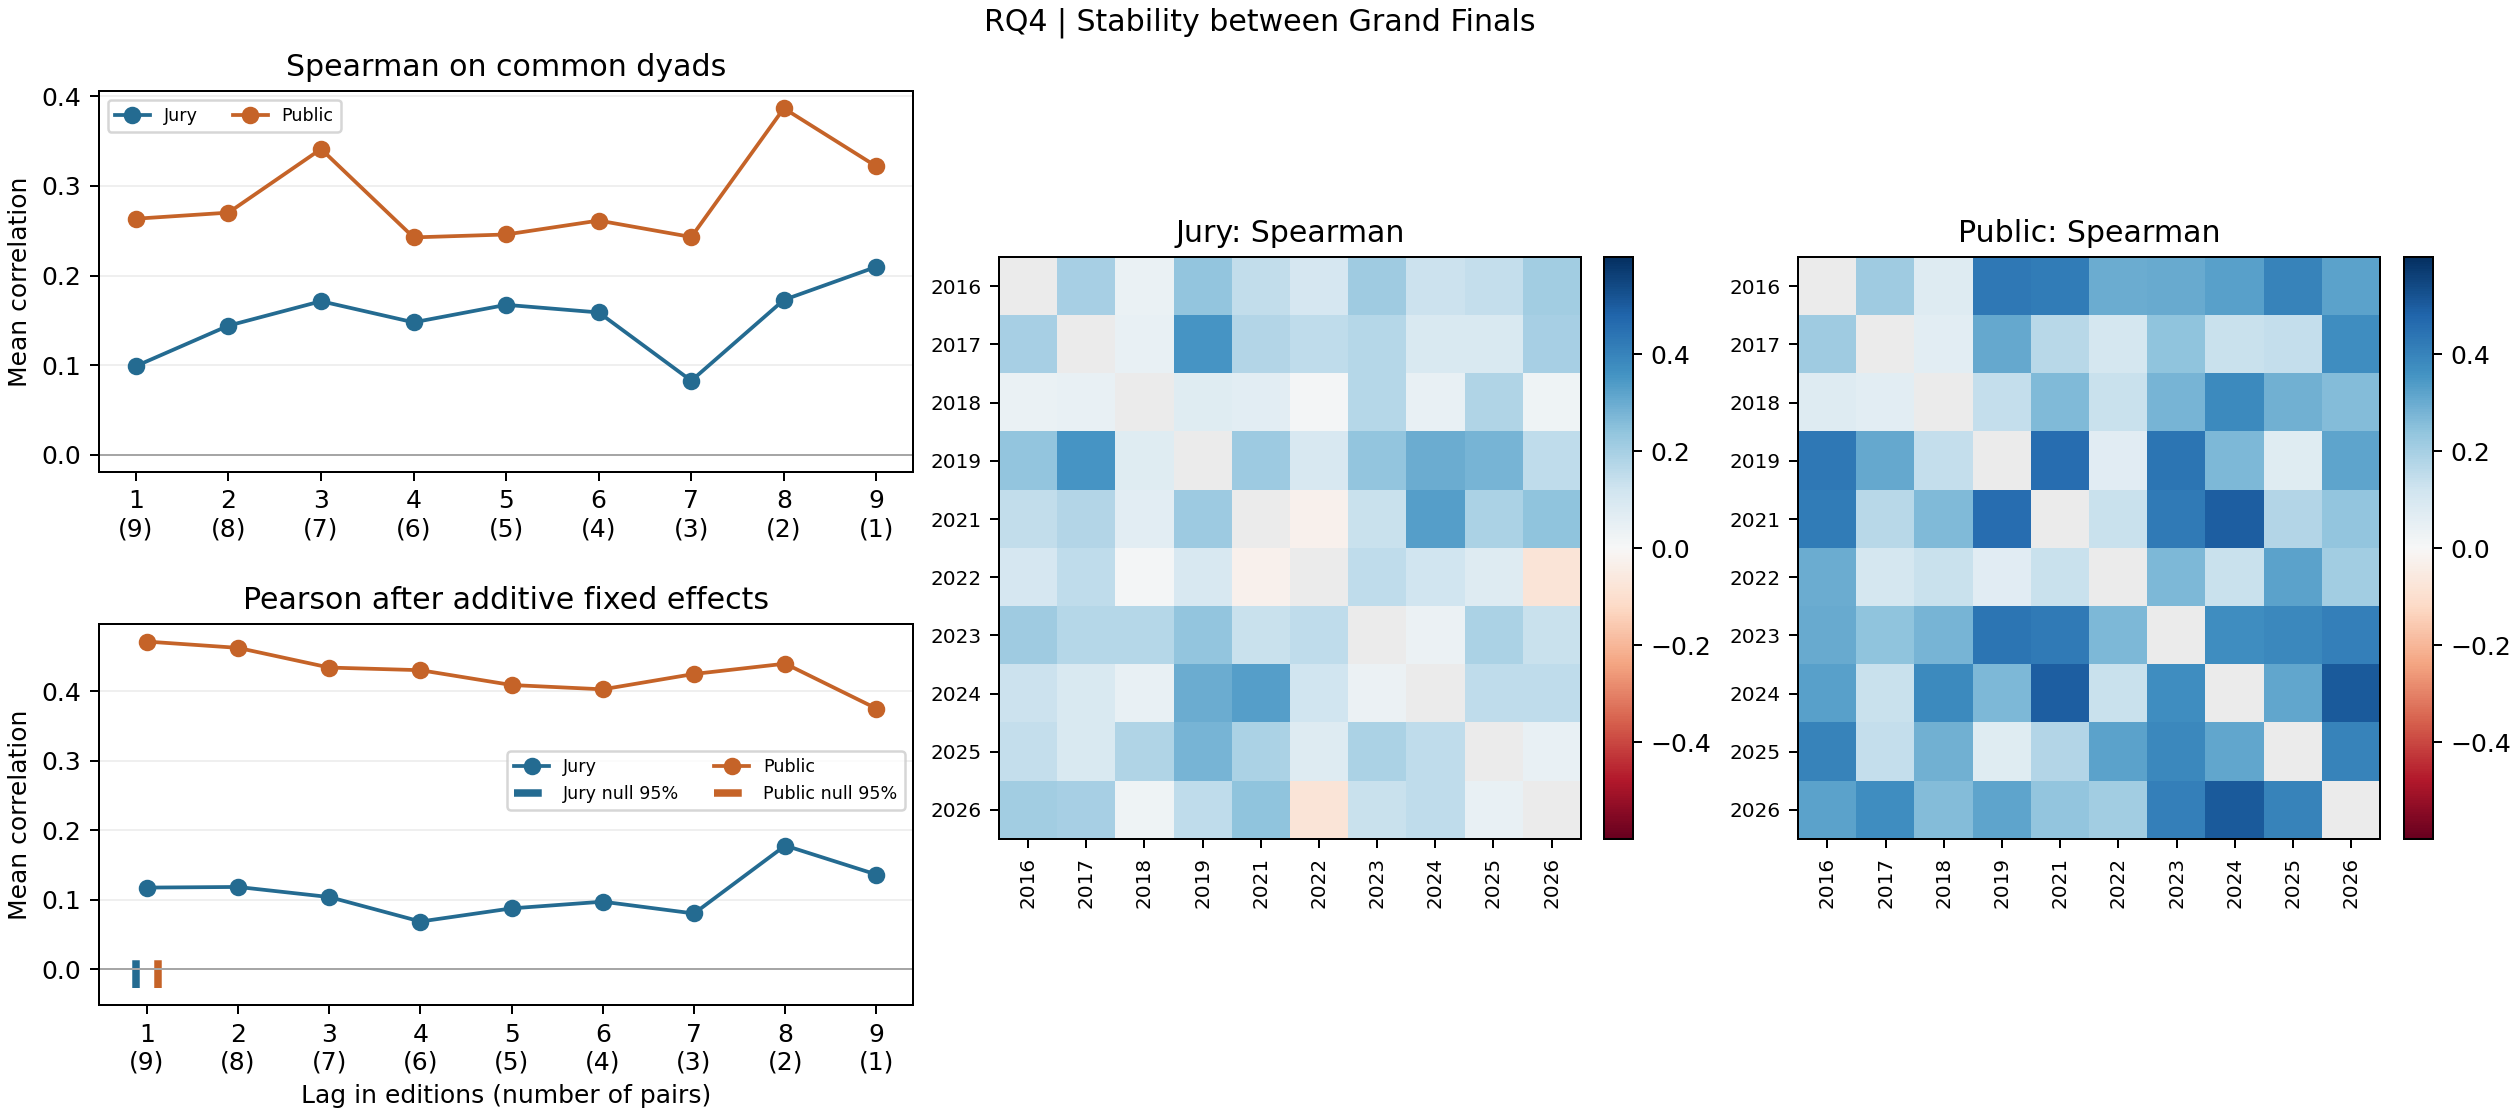
\includegraphics[width=\textwidth]
    {rq4_temporal_stability.png}
    \caption{Temporal similarity of jury and televote
    networks across Eurovision editions.
    The left panels show mean Spearman correlations
    and Pearson correlations after additive voter
    and recipient fixed effects, grouped by
    temporal lag. The right panels show pairwise
    Spearman correlations between editions.
    Public voting networks exhibit greater
    temporal similarity, especially in
    fixed-effect residual correlations.}
    \label{fig:rq4_temporal}
\end{figure}


% RQ5 - Prediction of strong votes


\subsection{RQ5: Predicting Strong Voting Ties}

RQ5 investigates whether geographical, linguistic,
and community information improves the prediction
of strong voting ties once historical voting
patterns and recipient popularity are considered.

For each voter and voting layer, the task is to
rank eligible finalists and predict the three
recipients of the highest scores (8, 10, and 12
points). We use an expanding-window evaluation,
training exclusively on previous editions and
testing on the 2023--2026 finals. This prevents
information from the target edition from entering
historical features or community detection.

We compare a random reference, a simple historical
ranking baseline, and four nested L2-regularised
logistic models \cite{hastie2009}.
M0a uses historical recipient popularity.
M0b additionally incorporates previous dyadic
voting, accumulated points, and reciprocity.
M1 introduces geographical and linguistic
similarity, while M2 further includes Louvain
community membership and cohesion.
Communities are reconstructed using only the
available training history.

The main evaluation measure is Hit@3, complemented
by NDCG@3 and mean reciprocal rank (MRR).
Table~\ref{tab:rq5_results} reports Hit@3 averaged
across the four test editions.

\begin{table}[htbp]
\centering
\caption{Mean Hit@3 across the 2023--2026 finals.}
\label{tab:rq5_results}
\small
\begin{tabular}{lcc}
\hline
Model & Jury & Public \\
\hline
Random reference & 0.1210 & 0.1210 \\
History baseline & 0.2461 & 0.4160 \\
M0a: Popularity & 0.2344 & 0.2103 \\
M0b: + Voting history & 0.2461 & 0.4273 \\
M1: + Geography/language & \textbf{0.2553} & 0.4297 \\
M2: + Communities & 0.2441 & \textbf{0.4322} \\
\hline
\end{tabular}
\end{table}


\begin{figure}[htbp]
    \centering
    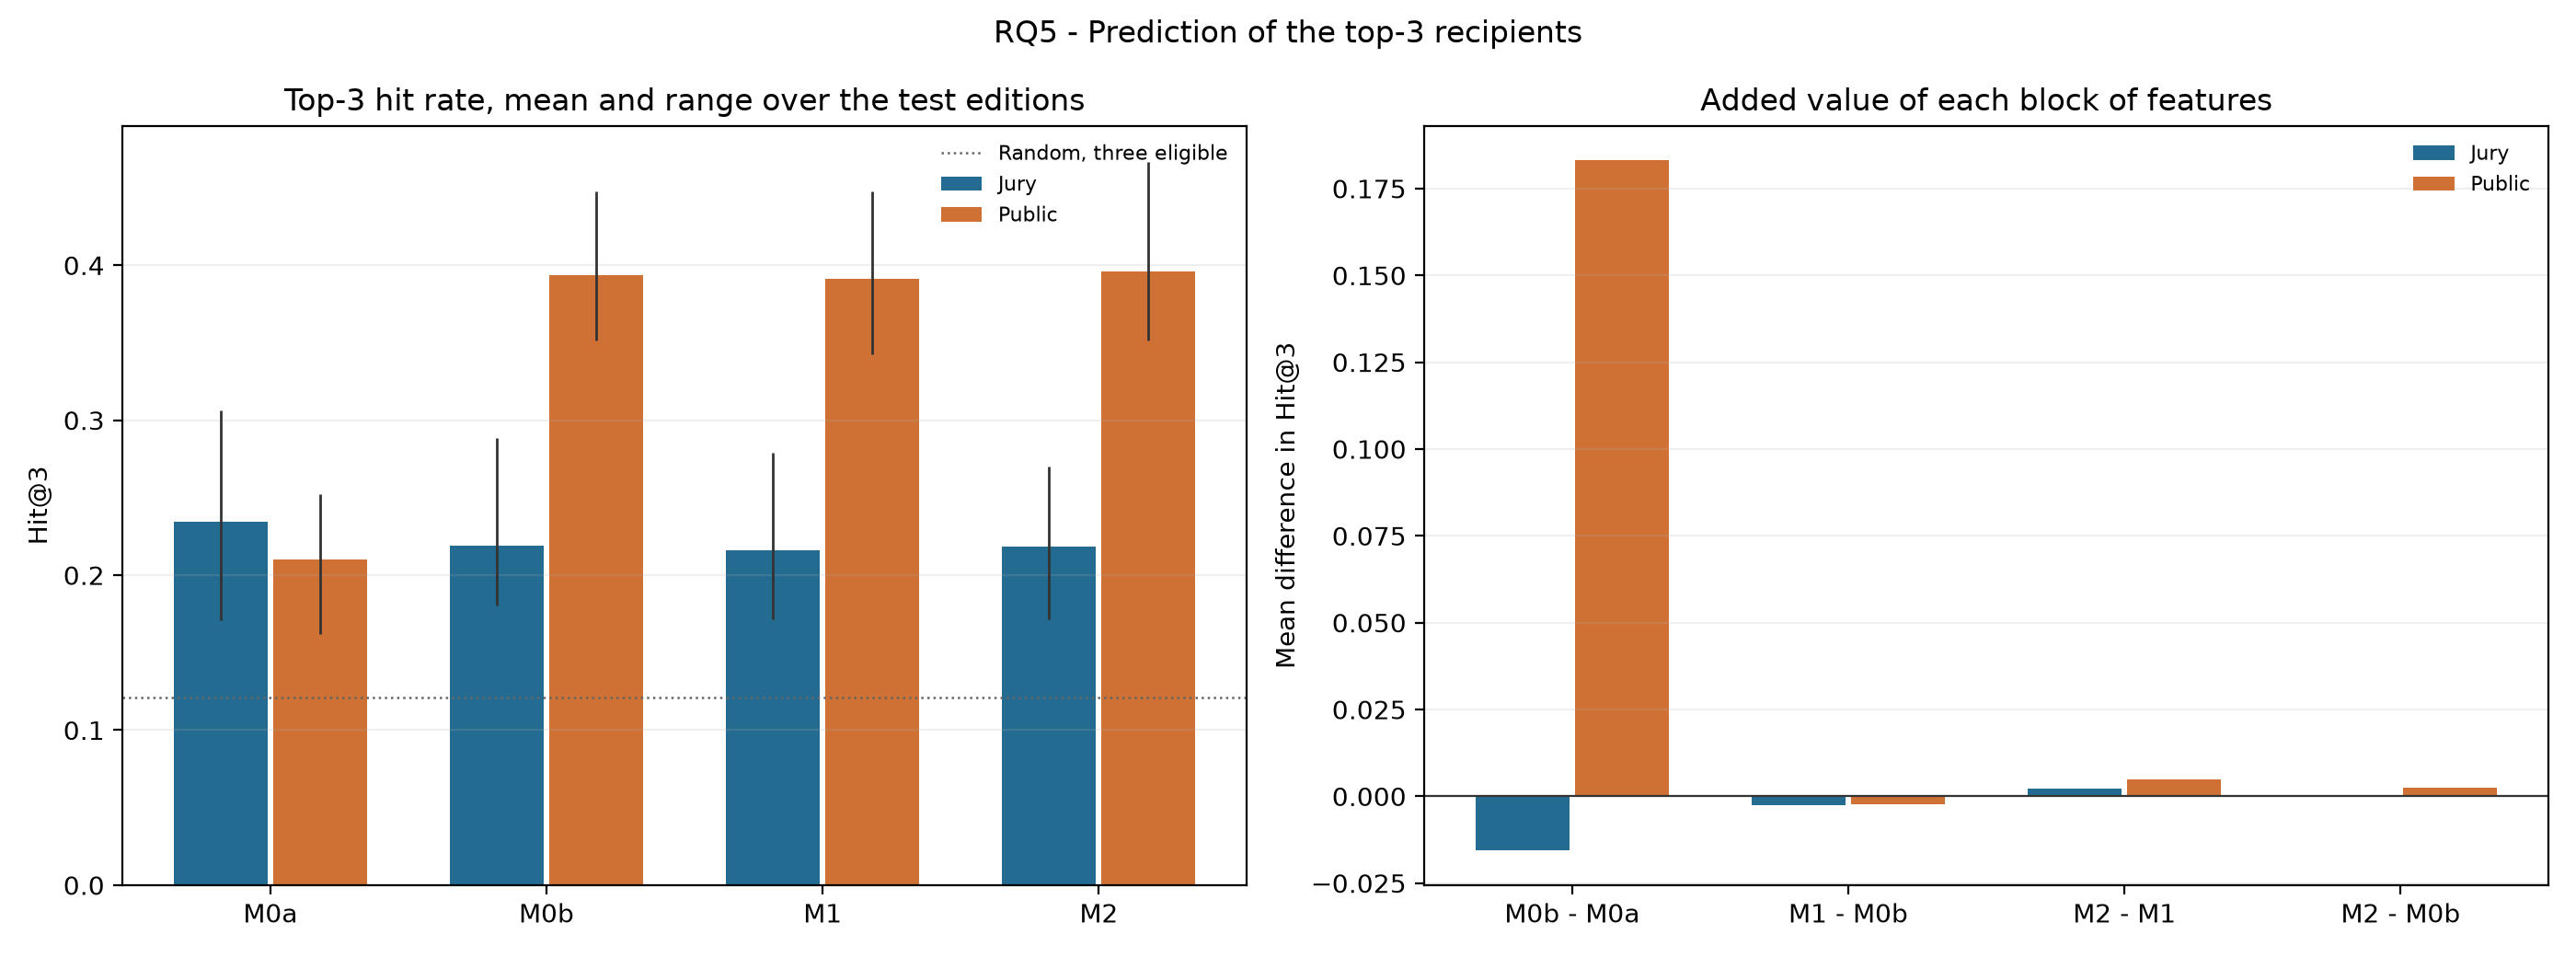
\includegraphics[width=\textwidth]
    {rq5_hit3_by_model.png}
    \caption{Hit@3 performance for predicting the
    three highest-scoring recipients in the
    2023--2026 Eurovision finals. Colored points
    represent individual test editions, black
    horizontal markers indicate the mean across
    editions, and the dashed horizontal line
    denotes the random baseline. Results are
    shown separately for jury and national
    televote predictions.}
    \label{fig:rq5_hit3}
\end{figure}


Figure~\ref{fig:rq5_hit3} shows that the
predictive advantage of voting history is
particularly pronounced in the public layer.
Although M2 achieves the highest average
public Hit@3, its improvement over M0b is
small and varies across test editions.


Historical voting information provides the
largest improvement for public voting.
Adding dyadic history to popularity increases
mean Hit@3 from 0.2103 (M0a) to 0.4273 (M0b).
By contrast, geography and language raise
public Hit@3 by only 0.0024, while Louvain
community features add another 0.0025.

For juries, the differences are smaller and
less consistent. M1 achieves the highest mean
Hit@3 (0.2553), whereas M2 falls to 0.2441.
Thus, additional community features do not
consistently improve predictions once voting
history and contextual attributes are included.

The historical baseline also performs strongly,
particularly for the public layer (0.4160),
indicating that much of the useful predictive
information is already present in repeated
voting relationships.

Robustness checks include leave-one-edition-out
comparisons, separate evaluations of previously
observed and unseen dyads, and deterministic
tie-breaking. All 40 fitted models converged.
A sensitivity analysis using Louvain consensus
over 200 initializations changes the mean M2
Hit@3 by only +0.0023 for juries and -0.0068
for the public.

Overall, the findings suggest that historical
dyadic relationships are substantially more
informative for public voting than recipient
popularity alone. Geographical, linguistic,
and community features provide limited
additional predictive value. Because the
evaluation covers only four test editions,
these differences remain descriptive rather
than evidence of general predictive superiority.

% ============================================
% 6. CONCLUSION
% ============================================

\section{Conclusion}
\label{conclusion}

The analysis of twenty Eurovision voting networks
reveals systematic differences between jury and
televote behaviour. Across the ten editions,
the public voting layer generally exhibits
stronger geographical preferences, greater
concentration of received points, and more
persistent voting relationships.

The five research questions provide complementary
perspectives on these patterns. RQ1 identifies
stronger high-score reciprocity and temporal
persistence in the televote, while showing
that some differences in triadic closure
can be explained by recipient popularity.
RQ2 reveals stronger geographical homophily
and greater correspondence between voting
communities and geographical groups in the
public layer. RQ3 confirms that public support
is more concentrated and more dependent on
within-region voting relationships.

RQ4 further demonstrates that both voting
systems exhibit temporal regularities, with
the televote showing substantially greater
similarity across consecutive editions.
These differences remain visible after
controlling for additive voter and recipient
effects and under the examined robustness
checks.

The predictive analysis in RQ5 connects
these structural observations to future
voting behaviour. Historical voting
relationships provide substantial predictive
information for the televote, whereas the
additional contributions of geographical,
linguistic, and community-based features
appear smaller and less consistent across
the observed test editions.

An important methodological finding is that
not every apparent network pattern represents
an independent structural effect. Several
observed relationships, particularly those
involving transitivity and the geographical
diversity of support, can arise partly from
recipient popularity and voting constraints.
Appropriate null models are therefore
essential for interpreting network measures.

Overall, the project highlights a fundamental
distinction between describing historical
network structures and demonstrating their
predictive usefulness. While geographical
and community patterns help characterise
Eurovision voting behaviour, their presence
does not necessarily imply additional
predictive value beyond historical voting
relationships.

These conclusions concern the editions
analysed and the assumptions of the
corresponding statistical models, rather
than establishing causal explanations
or universal voting behaviours.


% ============================================
% 7. CRITIQUE
% ============================================


\section{Critique}
\label{critique}

The study presents several limitations concerning
data representation, methodological assumptions,
and the generalisability of its findings.

First, Eurovision voting networks represent
countries rather than the individual songs
being evaluated. Musical genre, performance
quality, running order, artist reputation,
and other song-level characteristics are
not included. Consequently, observed
geographical preferences and persistent
voting relationships cannot be interpreted
as direct evidence of cultural affinity,
political alliances, or causal influences.
Future studies could incorporate song-level
features to separate these factors more clearly.

Second, geographical and linguistic attributes
are necessarily simplified. UN subregions
capture broad geographical relationships
but overlook physical distances, migration
patterns, and historical connections.
Similarly, language-family classifications
cannot fully represent multilingualism
or cultural proximity. More detailed
geographical distances and bilateral
migration data could provide alternative
explanations for observed voting patterns.

Third, the interpretation of network measures
depends on the selected null models.
Although the analyses account for important
constraints such as voting opportunities,
recipient popularity, and temporal dependence,
no single null model controls for every
possible source of structure. In particular,
the temporal permutation test in RQ4
evaluates persistence relative to a model
with exchangeable country identities,
rather than directly testing the equality
of two potentially persistent processes.

A further limitation concerns the number of
observations. The study covers ten editions,
and the predictive evaluation relies on
only four test finals. Although these
comparisons provide useful evidence,
the limited temporal sample restricts
statistical power and the generalisability
of predictive conclusions. Moreover,
consecutive editions share participating
countries and historical information,
introducing dependencies that complicate
conventional significance testing.

The predictive models also assume that
the finalist roster is known in advance.
Their performance therefore concerns the
ranking of eligible recipients, rather
than predicting the complete competition
outcome. Alternative approaches could
incorporate song-level covariates,
more flexible temporal models, and
additional historical editions.

Finally, the Rest of the World vote is
excluded because it cannot be associated
with an individual country. This ensures
consistency in country-level comparisons
but omits a component of the public
voting system from 2023 onwards.

Despite these limitations, the study
provides a reproducible comparison of
jury and televote networks and illustrates
the importance of distinguishing
descriptive network patterns from
statistically supported and
predictively useful relationships.

% ============================================
% REFERENCES
% ============================================

\begin{thebibliography}{99}

\bibitem{blondel2008}
Blondel, V. D., Guillaume, J.-L.,
Lambiotte, R., and Lefebvre, E. (2008).
Fast unfolding of communities in large networks.
\textit{Journal of Statistical Mechanics:
Theory and Experiment}, 2008(10), P10008.

\bibitem{danon2005}
Danon, L., D\'iaz-Guilera, A.,
Duch, J., and Arenas, A. (2005).
Comparing community structure identification.
\textit{Journal of Statistical Mechanics:
Theory and Experiment}, 2005(09), P09008.

\bibitem{eurovisionapi}
EurovisionAPI.
Eurovision Song Contest dataset.
\url{https://github.com/EurovisionAPI}.

\bibitem{ginsburgh2008}
Ginsburgh, V. and Noury, A. G. (2008).
The Eurovision Song Contest:
Is voting political or cultural?
\textit{European Journal of Political Economy},
24(1), 41--52.

\bibitem{hagberg2008}
Hagberg, A. A., Schult, D. A.,
and Swart, P. J. (2008).
Exploring network structure, dynamics,
and function using NetworkX.
\textit{Proceedings of the 7th Python
in Science Conference}, 11--15.

\bibitem{hastie2009}
Hastie, T., Tibshirani, R.,
and Friedman, J. (2009).
\textit{The Elements of Statistical Learning:
Data Mining, Inference, and Prediction}.
2nd ed., Springer.

\bibitem{projectrepo}
Botrugno, L., Fabrizio, D., Musa, S., and Samoggia, S. (2026).
Eurovision voting networks, 2016--2026: code, data and results.
\url{https://github.com/Samoggino/social-network-analysis}.

\bibitem{krackhardt1988}
Krackhardt, D. (1988).
Predicting with networks:
Nonparametric multiple regression
analysis of dyadic data.
\textit{Social Networks}, 10(4), 359--381.

\bibitem{newman2004}
Newman, M. E. J. and Girvan, M. (2004).
Finding and evaluating community structure.
\textit{Physical Review E}, 69(2), 026113.

\end{thebibliography}


\end{document}